\chapter{Thermometry of an ultracold Fermi gas}
\label{ch:idealfermigas}
The purpose of the camera is to measure distributions of atoms from which important physical quantities can be extracted. Dense atomic clouds consisting of Lithium and Caesium, the improvement of the resolution in the whole imaging setup now allows to explore new features that could not be detected before. As an example, the thermometry of an ultracold ideal Fermi Gases will be discussed in this chapter. At very low temperatures, the gas undergoes a phase transition from thermal into a degenerate state. This is reflected in the density distribution, which differs from a gaussian profile that one expects for a thermal gas.

These changes are small, nevertheless, they can be detected with the new setup. Therefore, this chapter starts with a brief introduction to absorption imaging in \refSec{absim}, which is used to image the atoms. Afterwards, the density distribution of ultracold, ideal Fermi gases in harmonic confinement are explained in \refSec{densdistrfermi}.
Finally, in \refSec{fermiexperiment}, the performed experiment with an ultracold gas of Li atoms and their analysis are presented.

\section{Absorption imaging}
\label{sec:absim}
In order to find microscopic properties of atoms, or assembles of atoms, it is necessary to look at the atoms themselves. This is commonly accomplished using either fluorescence or absorption imaging\cite{Murmann2011}. In both cases, a laser beam is pointed at an atomic cloud, that is cooled and confined in a trap. In fluorescence imaging, the scattered light is collected, typically in a direction that is different than the illuminating beam.
The intensity from the light reaching the detector is not very high, since it is radiated in all directions. Therefore, long exposure times are required during which atoms can move and the information about the initial density and energy distribution is lost. Nevertheless, this approach is useful for single- and few-atom detection.

In contrast, in absorption imaging\cite{helmrich2013}, the transmitted intensity of an imaging beam is recorded. Without atoms, one would detect the beam profile of the laser beam. With atoms, a shadow is visible due to the atoms "blocking" the light. This is accomplished, by correctly tuning the laser to a resonance frequency of the atoms, which enables them to absorb the light, exciting them to a higher state. Through spontaneous emission, the atoms will decay, making it possible to excite them once again. This method works well, when the "signal" from the absorbed light is significantly larger compared to the noise sources, and the atomic transition used for imaging is "closed", i.e. the excited atoms decay only into the imaging state.

In order to extract physical properties of the atoms after they have been illuminated, a quantity called optical density $OD$ is found in the absorption profile, which has an exponential dependency to the intensity reaching the CCD. From the optical density, one can conclude for example atomic distribution and atom numbers.
This is put into equations as follows:\cite{Murmann2011}
\begin{equation}
I_{CCD} = I_0 e^{-OD} + I_{back},
\end{equation}
which is decreasing from the initial intensity $I_0$ as the light is scattered by atoms. The intensity $I_{back}$ describes the background signal, that is found when the CCD is not being illuminated by a laser such as readout noise, dark noise or stray photon light. All the features of atoms are contained in the optical density, therefore in order to extract that, a background frame is subtracted from the absorption image and the laser profile divided, leaving
\begin{equation}
\frac{I_{CCD} - I_{back}}{I_0} = e^{-OD}.
\end{equation}
The laser intensity $I_0$ is measured in a separate frame, containing the laser intensiy $I_0' = I_0 + I_{back}$ and also the background $I_{back}$. Finally, for each pixel of the CCD detector, the equation yields
\begin{equation}
\frac{I_{CCD} - I_{back}}{I_0' - I_{back}} = e^{-OD}.
\end{equation}

From the resulting distribution of optical density, one can now extract, for example, atom density distributions, atom numbers or excitation rates.

\section{Density distribution of an ideal Fermi gas}
\label{sec:densdistrfermi}

An ideal Fermi gas consists of atoms, that all occupy the same internal state and are thus indistinguishable. This way, each energy level in the trapping potential is occupied by one or zero atoms up to the chemical potential $\mu$, so that the fermions do not interact with each other. This leads to a density distribution of the atoms, which, depending on the temperature $T$ and the chemical potential, can range between a common thermal distribution or a Fermi distribution for a degenerate cloud of atoms.

The fermionic cloud is characterized by the degeneracy parameter $T/T_F$, there $T_F$ is the Fermi temperature, which corresponds to the chemical potential for $T=0$. For values $T/T_F \gg 1$ the gas is then called thermal and will follow Maxwell-Boltzmann statistics. The cloud is called degenerate for $T/T_F \ll 1$ and the density profile will be a Fermi distribution. This is described by a shape parameter $q=\frac{\mu}{k_BT}$ with the Boltzmann constant $k_B$, which is large and negative in the thermal and large and positive in the degenerate regime. In this way, both the regimes are connected by contous tuning of $q$.

In order to find out if the cloud is thermal or degenerate, one can fit a distribution, that interpolates between both regimes. The following derivations can be found in \cite{Ketterle2008}.

In the Gaussian distribution, the width $\sigma_i$ is defined by
\begin{equation}
\sigma _i = \sqrt{\frac{2k_BT}{mw_i^2}},
\end{equation}
where $m$ is the mass of Lithium and $w_i$ is the trapping frequency in the $i=\{x,y,z\}$ direction of the cloud. Due to the alignment of the dipole trap, the cloud will not have a spherical shape and will therefore have different radii\cite{Heck2012}.

In the degenerate regime however, the atom density is best described by a Thomas-Fermi distribution with the Fermi radius
\begin{equation}
R_{Fi} = \sqrt{\frac{2E_F}{mw_i^2}},
\end{equation}
where $E_F=\hbar \bar{w} (6N)^{1/3}$ is the Fermi energy ($N$ being the number of atoms and $\bar{w}=(w_1 w_2 w_3)^{1/3}$ is the geometrically averaged trapping frequency).

Experimentally, it is very hard to prepare a purely degenerate Fermi gas, such that a typical density distribution will contain contributions also from the thermal fraction of atoms.
Therefore a unified radius,
\begin{equation}
R_i^2 = \frac{2k_BT}{mw_i^2}f( e^{q}),
\end{equation}
can be used, with the previously declared shape parameter $q$. It smoothly interpolates between the two regimes and is used in fitting the atom density distributions.
The interpolation function $f(x)$ is
\begin{equation}
f(x) = \frac{Li_1(-x)}{Li_0(-x)} = \frac{1+x}{x} ln(1+x),
\end{equation}
where $Li_n$ is the n-th order polylogarithm and can be defined as
\begin{equation}
Li_s(z) = \sum_{k=1}^{\infty} \frac{z^k}{k^s}.
\end{equation}

In our case, we integrate over all but one axes, and therefore the fitting function for the doubly integrated atom density distribution yields
\begin{equation}
\label{eq:n1d}
n_{1D}(x) = n_{1D,0}\frac{Li_{5/2}\left( \pm \mathrm{exp}\left[ q-\frac{x^2}{R_i^2}f(e^q)\right] \right)}{Li_{5/2}(\pm e^q)}.
\end{equation}
During fitting, the shape parameter $q=\frac{\mu}{k_B T}$ is extracted, which describes the ratio between chemical potential and thermal energy of the gas.

In order to calculate the degeneracy parameter $T/T_F$, the value of $q$ is inserted into the equation:
\begin{equation}
\label{eq:tovertf}
\frac{T}{T_F} = \left[ -6 Li_3(-e^q) \right]^{-1/3}.
\end{equation}

As the camera only has a finite resolution, the cloud can be released and imaged after a short time. At the time of the acqusition, the gas will have expanded, although the distribution is approximately the same. During expansion of the cloud, the temperature, which is dependent on the radius, will not change. Therefore, the radius is contracted in order to receive the radius of the inital distribution by
\begin{equation}
R_{0,i} = \frac{R_{i}}{\sqrt{1+ w_i^2}},
\end{equation}
which can then be used to calculate the temperature of the cloud using
\begin{equation}
\label{eq:temp}
T = \frac{1}{2} \frac{mw_i^2}{k_B} \frac{R_i^2}{1+w_i^2t^2}\frac{1}{f(e^q)}.
\end{equation}


	
\section{Preparation and imaging of an ultracold Fermi gas}
\label{sec:fermiexperiment}

In order to conduct an experiment involving an ideal Fermi gas, Lithium atoms were prepared using various traps. From a magneto-optical trap, the atoms were transferred into a D1 cooling and then loaded into an optical dipole trap. From there on, the fermions were further evaporatively cooled, by tuning the power of the dipole lasers. Naturally, the spins of the atoms are uniformly distributed, which helps with the evaporative cooling process, due to momentum transfers of the atoms. In order to create an ideal Fermi gas, one spin component is removed by resonantly exciting them with a laser pulse, which will not affect the other component, leaving them in the trap. Atoms were prepared for several trap depths in order to compare the results.

The cloud was imaged using the new camera system, yielding the results in \refFig{fermi_fit}. The atoms can be seen as a cloud which is slightly larger in x than in the y direction, which is due to the geometry of the optical dipole trap. The distributions along the x and y axis already have a gaussian shape which is discussed in the next step.

In order to extract the physical quantities, \refEq{n1d} was fitted, leaving $q$, $n_{1D,0}$ and $R_i$ free. The distribution along the x axis have fragments, which are most likely due to the alignment of the optical setup, which has not been refined as of the writing of this thesis. Therefore, the fit was included in the picture, but the fit parameters were not extracted as they are most likely not accurate. On the y axis, a linear gradient is visible. This is an effect of the readout of the chip and was fitted as well, but does not affect the physics as it does not interfere with the original function.

From the fit parameters, the temperature and degeneracy parameter were calculated, which are found in Table \ref{tab:fermi_fit}. Additionally, a temperature $T_{tof}$ was calculated by taking a time of flight measurement from a different camera, which relates the linear expansion to the velocity and therefore to the temperature of the gas.

From the results, we find that there is a match between the temperatures, although the temperature extracted from the original fit is probably better, since it includes the degenerate fraction as well. This is especially true for the two lower trap frequencies, where the shape parameter $q$ indicates that the cloud is more degenerate than thermal.

\pltCustom{
	\begin{center}
		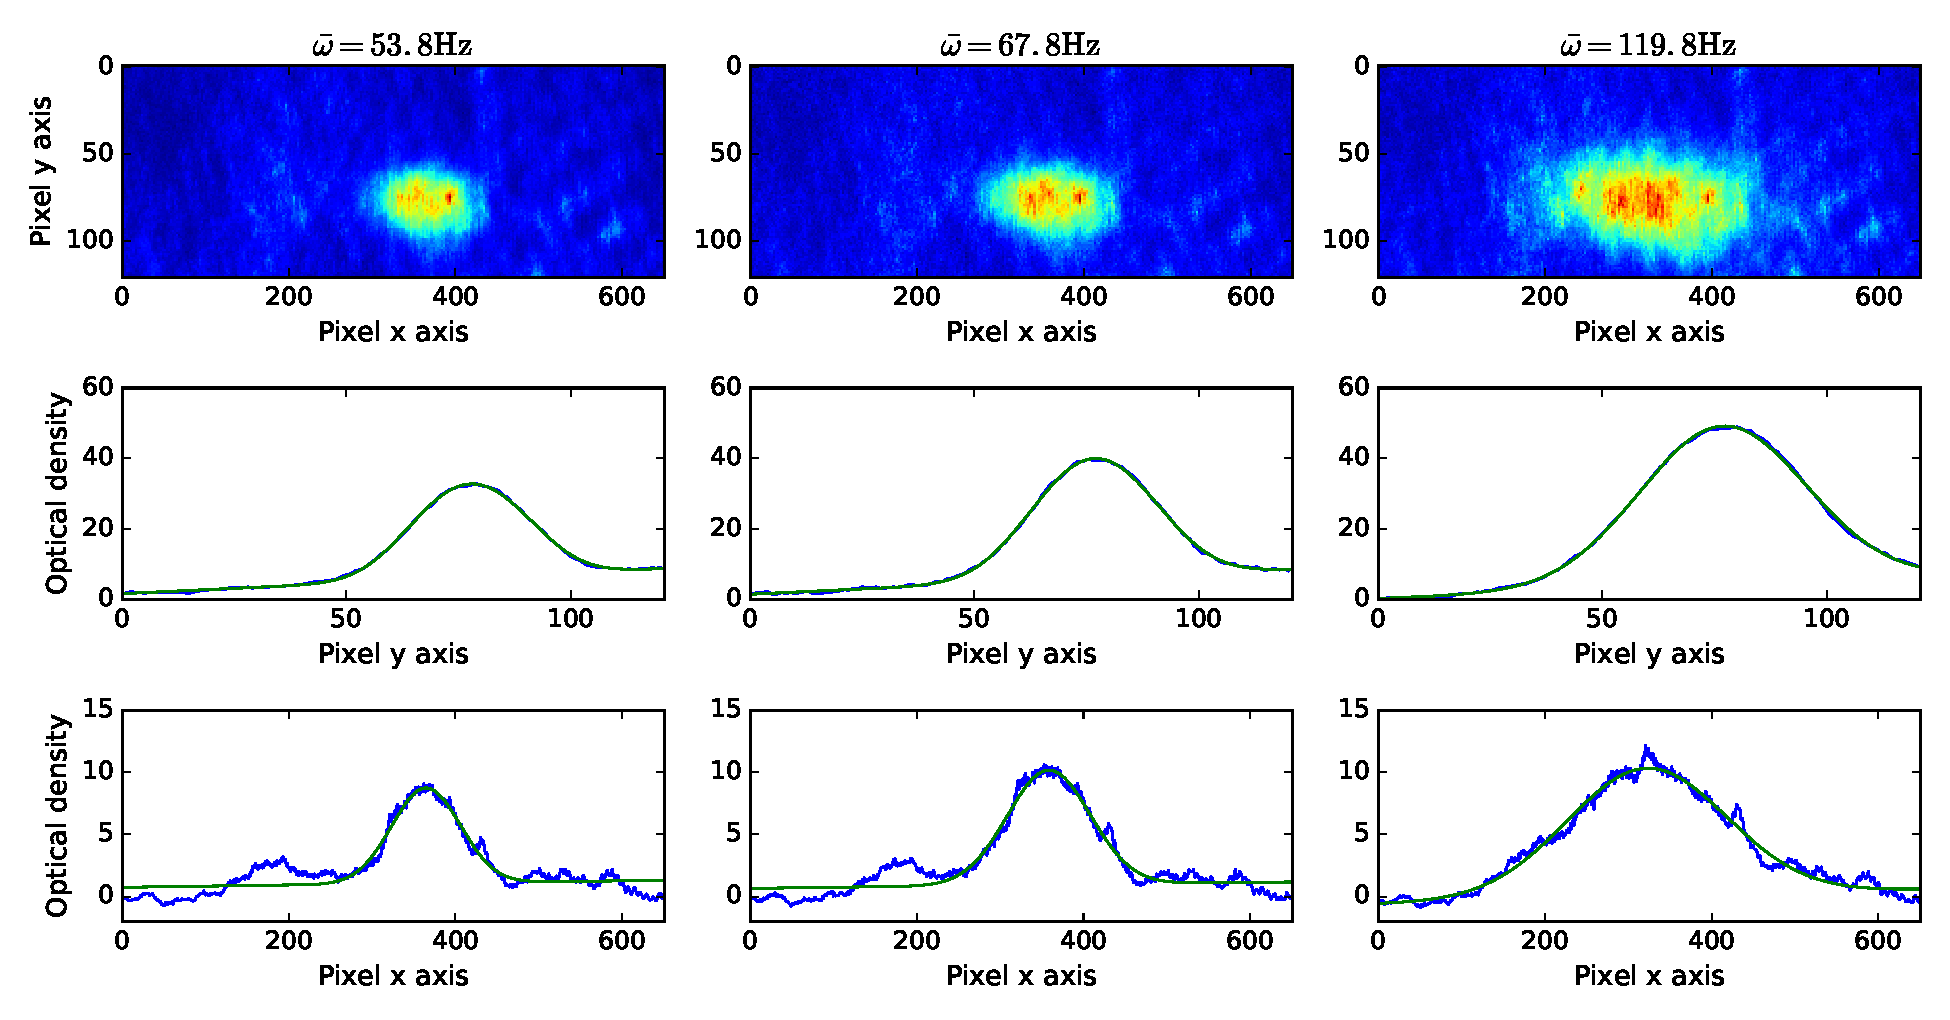
\includegraphics[width=1\textwidth]{drafts/fermi_fit.pdf}
	\end{center}
	\begin{textblock}{2}(0.75,-4.7)
		\textbf{a.}
	\end{textblock}
	\begin{textblock}{2}(4.55,-4.7)
		\textbf{b.}
	\end{textblock}
	\begin{textblock}{2}(8.35,-4.7)
		\textbf{c.}
	\end{textblock}
}{fermi_fit}{Fitting the Fermi distribution to an ultracold gas of Li atoms}{In order to find the physical properties of a fermionic cloud, they were imaged at three different trap depths which correspond to the $\bar{\omega} = (\omega_x \omega_y \omega_z)^{1/3}$, where $w_i$ is the trap frequency in the corresponding axis. As of the writing of this thesis, the imaging system was not yet well aligned in the x-Direction, therefore the data does not represent the theory well. The results of the fits are given in Table \ref{tab:fermi_fit}.}

\begin{table}
	\begin{center}
		\begin{tabular}{M{1.5cm}!M{4cm}|M{4cm}|M{4cm}N}
			& $\bar{\omega}=\SI{53.8}{\hertz}$ & $\bar{\omega}=\SI{67.8}{\hertz}$ & $\bar{\omega}=\SI{119.8}{\hertz}$ & \\[7pt]
			\thickhline
			$n_{1D}$ & $25.6\pm0.1$ & $34.07\pm0.13$ & $44.98\pm0.24$ & \\ [7pt]
			\hline
			$q$ & $1.87\pm0.35$ & $1.08\pm0.34$ & $-2.0\pm1.85$ & \\[7pt]
			\hline
			$R_y [\SI{}{\micro\meter}]$ & $41.4\pm1.3$ & $41.3\pm1.3$ & $46.4\pm1.8$ & \\[7pt]
			\hline
			$T [\SI{}{\nano\kelvin}]$ & $59.2\pm2.5$ & $117.4\pm3.7$ & $536\pm77$ & \\[7pt]
			\hline
			$T/T_F$ & $0.34\pm0.11$ & $0.42\pm0.04$ & $1.01\pm0.41$ & \\[7pt]
			\hline
			$T_{tof} [\SI{}{\nano\kelvin}]$ & $56$ & $97$ & $480$ & \\[7pt]
		\end{tabular}
	\end{center}
	\setCaption{Fit parameters for various trap depths}{The Fermions were fitted using \refEq{n1d}, where the parameter $n_{1D}$ describes the amplitude of the peak. $q$ is a shape parameter, which is negative if the cloud is thermal or positive if the cloud is degenerate. $R_y$ is then the clouds radius similar as the radius can be described in a gaussian distribution which is in units of pixels and can be calculated in natural units using the pixel size (\SI{13}{\micro\meter}) and the magnification ($7.5$).}
	\label{tab:fermi_fit}
\end{table}